\section{Red Cross}

\begin{figure}[htbp]
\centering
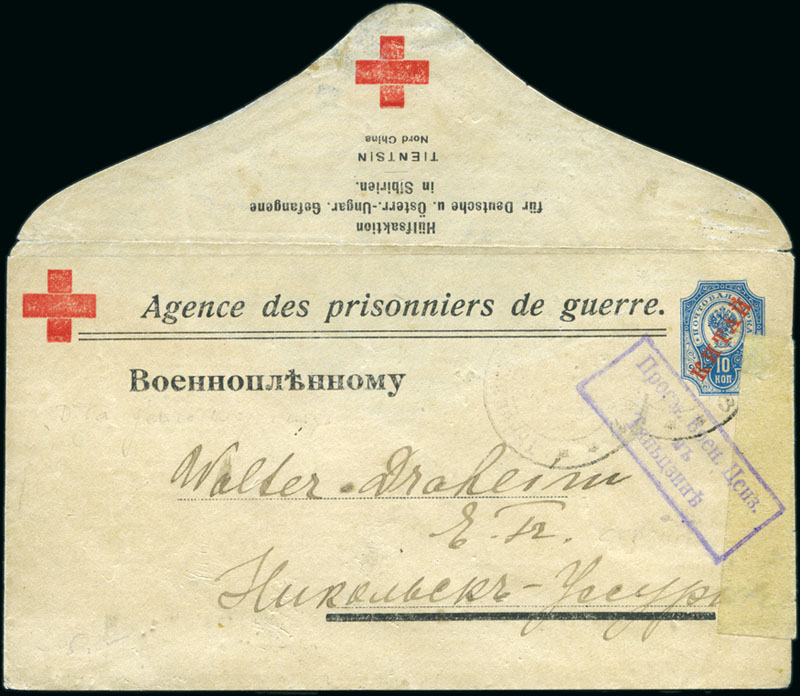
\includegraphics[width=.95\textwidth]{../russian-post-offices-in-china/10016.jpg}
\caption{
10016	TIENTSIN: "KITAI" 10k postal stationery envelope printed for used by
the Red Cross P.O.W. Agency, lightly cancelled by Tienstin cds (T\&S type 6), 
with violet boxed "Examined Military Censor / In / Tienstin" censor hs adjacent, 
fine.
Note: Origin of the illustration in "Russische Postcensuur 1914-1918" p.94
by A. Speeckaert
\euro 400.00
}  
\end{figure}

\begin{figure}[htbp]
\centering
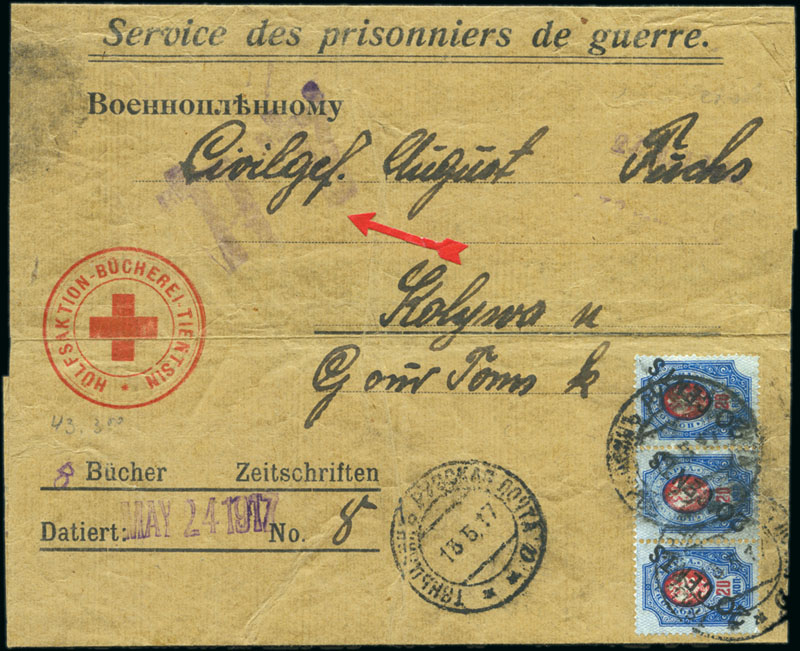
\includegraphics[width=.95\textwidth]{../russian-post-offices-in-china/10017.jpg}
\caption{
10017	TIENTSIN: 1917 Prisoner of War printed wrapper sent from a German P.O.W. 
Relief Agency used to send reading matter to a P.O.W. in Kolyvan (Siberia), 
franked with Chinese surcharged 20c on 20k strip of three, all tied by 
Tientsin 13.5.17 cds (T\&S type 6), with censored hs applied at Tientsin on 
obverse (unrecorded type)
\euro 400.00
}  
\end{figure}

\begin{figure}[htbp]
\centering
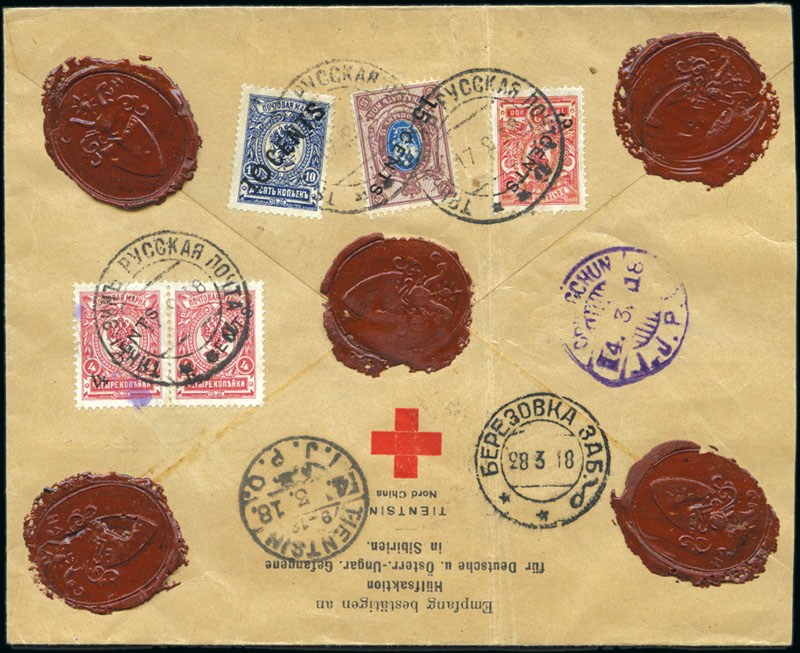
\includegraphics[width=.95\textwidth]{../russian-post-offices-in-china/10019.jpg}
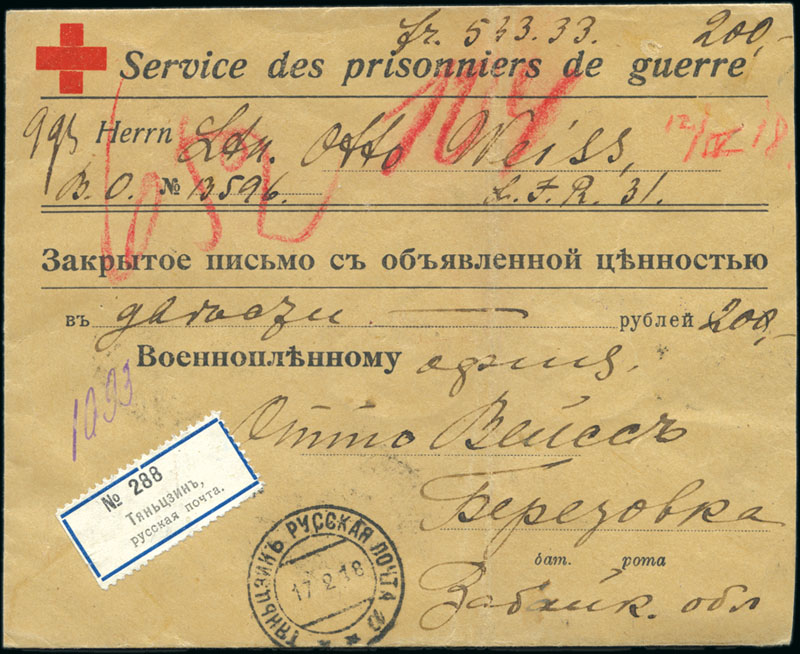
\includegraphics[width=.95\textwidth]{../russian-post-offices-in-china/10019-1.jpg}
\caption{
10019 TIENTSIN: 1918 Prisoner of War printed envelope sent insured for 200R
to P.O.W. at Berezovka (Siberia), franked on the reverse with 3c on 3k, 4c on 4k (2),
10c on 10k and 15c on 15k all tied by Tientsin 17.2.18 cds (T\&S type 6), 
sent via the Japanese P.O.s at Tientsin and Changchun, with insured label on 
obverse, wax seals on reverse, attractive.
\euro 300.00
}  
\end{figure}




                                                                  